\documentclass[t,aspectratio=169]{beamer}

\usepackage{bm}
\usepackage{soul}
\usepackage{tikz}
\usepackage{tikz-3dplot}
\usepackage{amsmath}
\usepackage{amsfonts}
\usepackage{amssymb}
%\usepackage{physics}
%\usepackage{graphicx}
\usepackage{multicol}
\usepackage{t1enc}
\usepackage[utf8]{inputenc}
\usepackage[magyar]{babel}
\usepackage{pgfplots}
\pgfplotsset{compat=1.18}


\usetikzlibrary{calc,3d,decorations.pathmorphing,decorations.pathreplacing,decorations.markings,snakes,arrows.meta,calc,patterns
}
\tikzset{snake it/.style={decorate, decoration=snake}}
% \usetheme{Madrid}
% \usecolortheme{whale}

%\usepackage{hyperref}
\hypersetup{
    colorlinks=true,
    linkcolor=blue,
    filecolor=magenta,      
    urlcolor=cyan,
    pdftitle={(KTXFI1EBNF) Physics I. Lecture},
}

% ----------------------------------------------------------------------------------------------------------------------------------------

\title{\includegraphics[width=45pt]{oepecsetlogo.png}\\(KTXFI1EBNF) Physics I. Lecture}

\author{Dr.~Gábor FACSKÓ, PhD\\\tiny Assistant Professor / Senior Research Fellow\\\textit{facsko.gabor@uni-obuda.hu}}

\institute{\Tiny Óbuda University, Faculty of Electrical Engineering, 1084 Budapest, Tavaszmező u. 17.\\Wigner Research Centre for Physics, Department of Space Physics and Space Technology, 1121 Budapest, Konkoly-Thege~Miklós~út~29–33.\\ \url{https://wigner.hu/~facsko.gabor}}

\date{March~30,~2026}

\logo{\includegraphics[height=0.9 true cm]{kekcsik.png}}

% ----------------------------------------------------------------------------------------------------------------------------------------

\begin{document}

\frame{\titlepage}

% ----------------------------------------------------------------------------------------------------------------------------------------

\begin{frame}
\frametitle{Current Updates and Issues}
\begin{itemize}
\setlength{\parskip}{0pt}
\setlength{\itemsep}{4pt}
\item Thank you for submitting your first homework assignment. I have graded the papers and provided the solutions. Three students did not submit their assignments; therefore, I must deny their signatures.
\item I found errors in the material. Specifically, the direction of the force vectors and their starting points were not always correct. I have corrected these mistakes. 
\item The dates of the exams are not final. Let me know if you need more time or a different schedule. 
\item Future: we will finish Thermodynamics during this lecture. I will need more time for the practical part of this field. Then you will receive your 2nd assignment.
\item \st{Electrodynamics} Electrostatics: no previous material available for lectures. Some mid-term exam exercises are available $\rightarrow$ We will practice them, and I will use my creativity. 
\end{itemize}
\end{frame}

% ----------------------------------------------------------------------------------------------------------------------------------------

\begin{frame}[fragile,squeeze,allowframebreaks]
\frametitle{Where are we?}
\begin{enumerate}
\setlength{\parskip}{0pt}
\setlength{\itemsep}{0pt}
\item \textbf{Mechanics I.:} Newton’s laws, equation of motion (review). Momentum. General concept of mechanical work, work theorem. Forms of mechanical energy.
\item \textbf{Mechanics II.:} Weight force, gravitational force, gravitational field. Work of the gravitational force. Conservative force field. Dissipative force field. Mechanical power.
\item \textbf{Mechanics of Rigid Bodies I.} Concept of a rigid body. Forces acting on a rigid body. Motion of a rigid body. Concept of the centre of mass. Location of the centre of mass. Torque. Angular momentum. Energy of a rotating rigid body, angular momentum of a rotating rigid body, Steiner’s theorem.
\item \textbf{Mechanics of Rigid Bodies II.} Principal theorems of rigid body motion; conservation laws. Collisions.
\item \textbf{Oscillations I.} Dynamic condition of harmonic oscillatory motion. Differential equation of harmonic undamped oscillatory motion.
\pagebreak
\item \textbf{Oscillations II.} Superposition of oscillations. Decomposition of oscillations into components. Damped oscillations. Forced oscillations, resonance. Coupled oscillations.
\item \textbf{Wave phenomena:} Reflection of waves, refraction of waves, diffraction of waves. Huygens–Fresnel principle. Interference of waves. Polarization of waves.
\item \textbf{Elements of acoustics:} Basics of acoustics. Fundamental concepts. Doppler effect. Sound intensity, loudness according to Weber–Fechner’s law.
\item \textbf{Thermodynamics I:} Temperature scales, thermal expansion, thermometers. State variables, ideal gas, state changes, ideal gas equation of state, Boyle’s law, Gay-Lussac’s laws, universal (combined) gas law, heat, specific heat, molar heat, heat capacity.
\item \textbf{Thermodynamics II:} Expansion work, internal energy, the first law of thermodynamics, forms of the first law in different state changes.
\pagebreak
\vskip -10 pt
\item \textbf{Thermodynamics III:} Cyclic processes, Carnot cycle, Carnot’s theorem, reduced heat, entropy, the second law of thermodynamics.
\item \textbf{Thermodynamics IV:} \textit{Kinetic theory of gases, molecular thermodynamics. Distributions, distribution functions. Elementary statistics.}
\item \textbf{Electrostatics I.:} Electric charge: Fundamental electrical phenomena, electric charge and matter, Coulomb’s law (force between two point charges, unit of electric charge, permittivity of vacuum).
\item \textbf{Electrostatics II.:} The electric field: The electrostatic field (electric field strength, electric field lines). Determination of electric field strength. Gauss’s law (flux of the electric field). Electric field of a point charge.
\pagebreak
\item \textbf{Electrostatics III.:} Electrostatic potential: Work of the electric field (work done in an electric field). Electric potential (electrostatic potential). Electric potential difference, voltage. Electric potential of charge systems at small and large distances. Electrostatic energy.
\item \textbf{Elements of physical or wave optics.} Branches of optics. Light interference, light diffraction, diffraction through a slit, optical grating, light polarization. Light as an electromagnetic wave: Poynting vector. Optical instruments.
\end{enumerate}
\end{frame}

% ----------------------------------------------------------------------------------------------------------------------------------------

\begin{frame}[fragile,squeeze,allowframebreaks]
\frametitle{Kinetic gas theory}

\begin{itemize}
\setlength{\parskip}{0pt}
\setlength{\itemsep}{4pt}

\item Interpretation of the main thermodynamic quantities based on kinetic gas theory

\item Pressure: $p = \frac{1}{3} \rho \overline{v^2}$ where $\overline{v^2}$ is the mean of $v^2$.

\item Ideal gas equation of state: $$pV = \frac{m}{M} RT$$
$m = N \cdot m_0$, where $m$: mass of the gas, and $m_0$: mass of one particle \\
$M = N_A \cdot m_0$, where $M$ is the molar mass

\item \textbf{Definition (Avogadro's number):} $$N_A = 6 \cdot 10^{23}$$

\pagebreak
\item According to these:
$$pV = \frac{N m_0}{N_A m_0} RT = N \frac{R}{N_A} T$$

\item \textbf{Definition (Boltzmann's constant):}
$$k = \frac{R}{N_A}$$

\item Hence,
$$pV = NkT$$

\pagebreak
\item The interpretation of temperature
\vskip -20 pt
\begin{eqnarray*}  
p = \frac{1}{3} \rho \overline{v^2} &=& \frac{1}{3} \frac{N m_0}{V} \overline{v^2} \cdot V\\
pV &=& \frac{1}{3} N m_0 \overline{v^2}
\end{eqnarray*}
\item From previously: $pV = N k T$. Therefore,
\vskip -20 pt
\begin{eqnarray*}
\frac{1}{3} N m_0 \overline{v^2} &=& N k T \quad : N \\
\frac{1}{3} m_0 \overline{v^2} &=& k T \quad \cdot 3 \\
m_0 \overline{v^2} &=& 3 k T \quad : 2 \\
\frac{1}{2} m_0 \overline{v^2} &=& \frac{3}{2} k T
\end{eqnarray*}
  
\framebreak

\item Equipartition theorem: each degree of freedom of a gas molecule has the same amount of kinetic energy, which is equal to $\frac{1}{2} k T$.

\item $\frac{1}{2} m_0 \overline{v^2}$ can be divided into 3 parts: according to the x, y, z coordinates. Hence,
$$\frac{3}{2} m_0 \overline{v_i^2} = \frac{3}{2} k T \implies \frac{1}{2} m_0 \overline{v_i^2} = \frac{1}{2} k T$$

\item If the number of degrees of freedom is $f$: 
$$\frac{1}{2} m_0 \overline{v_i^2} = \frac{f}{2} k T$$

\framebreak
\item Internal energy of ideal gas:
$$U = N \frac{1}{2} m_0 \overline{v^2} = N \frac{f}{2} k T$$

\item Specific heat and molar heat:
$$U = c_v m T = N \frac{f}{2} k T = \frac{f}{2} \frac{m}{M} R T$$

\item From the equation the $c_v$ can be expressed:
\begin{eqnarray*}  
c_v m T &=& \frac{f}{2} \frac{m}{M} R T \\
c_v &=& \frac{f}{2} \frac{R}{M} = \frac{f}{2} R_i \\
C_V &=& c_v M = \frac{f}{2} R\\
c_p &=& c_v + \frac{R}{M} = \frac{R}{M} (\frac{f}{2} + 1)\\
C_p &=& C_V + R = (\frac{f + 2}{2}) R
\end{eqnarray*} 
  
\framebreak
\item Boltzmann’s definition of entropy: $$S = k \cdot \ln w,$$ where $w$: number of microstates associated with a macrostate (thermodynamic probability), and $k$ is Boltzmann-constant.

\item The change in entropy according to Boltzmann’s interpretation:
$$\Delta S = k \cdot \ln \frac{w_2}{w_1}.$$

\item The change in entropy for ideal gas state changes:
\vskip -10 pt
$$\Delta S = \int_{T_1}^{T_2} \frac{c_v m \, dT}{T} + \int_{V_1}^{V_2} \frac{m R_i}{V} \, dV = c_v m \ln \frac{T_2}{T_1} + m R_i \ln \frac{V_2}{V_1}$$

\end{itemize}

\framebreak

\begin{center}
\includegraphics[width=0.6\textwidth]{images-20260330/boltzmann.png}
\end{center}

\end{frame}

% ----------------------------------------------------------------------------------------------------------------------------------------


\begin{frame}[fragile,squeeze,allowframebreaks]
\frametitle{Thermodynamic distributions}

\begin{itemize}
\setlength{\parskip}{0pt}
\setlength{\itemsep}{4pt}

\item Spatial distribution: $$n_i = n_0 \cdot e^{\frac{-W_i}{kT}},$$ where $n_i$: number of particles in the i-th state, $n_0$: reference number of particles, usually representing the number in the most probable or ground state, $W_i$: the energy of the i-th state.

\item Velocity distribution: 
$$\rho(v) = \frac{dn}{dv} = 4\pi \left( \frac{m_0}{2\pi kT} \right)^{3/2} v^2 e^{\frac{-m_0 v^2}{2kT}},$$
where $\rho(v)$: the probability density function of the velocity distribution, $\frac{dn}{dv}$: the velocity density, showing how particles are distributed across different velocities. $m$ is the mass of the particles. $v$ is the velocity of the particles.


\framebreak
\item Velocity Distributions at Different Temperatures
\smallskip
\begin{center}
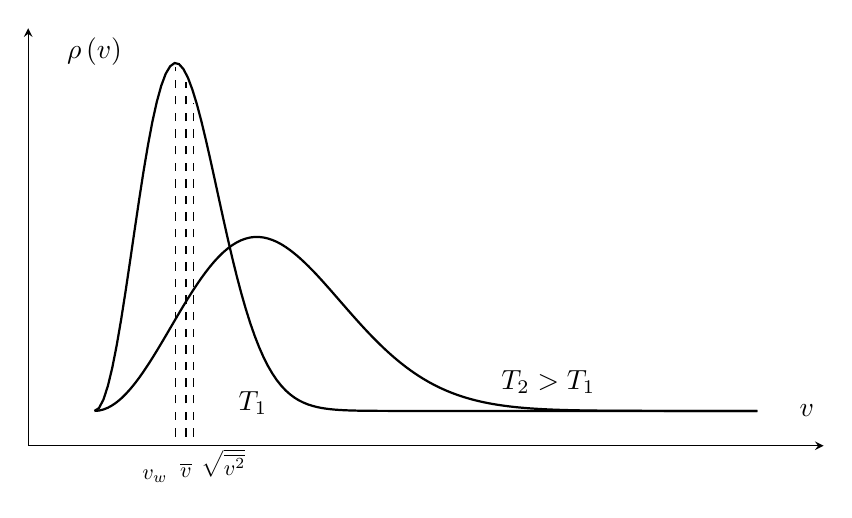
\begin{tikzpicture}
\begin{axis}[
    axis lines = left,
    xlabel = {$v$},
    ylabel = {$\rho\left(v\right)$},
    domain = 0:10,
    samples = 150,
    ytick = \empty,
    xtick = \empty,
    enlargelimits = true,
    clip = false,
    width = 10cm,
    height = 6cm,
    every axis x label/.style={at={(current axis.right of origin)},anchor=east},
    every axis y label/.style={at={(current axis.above origin)},anchor=north},
scale=1.2]
    % T2: Magasabb hőmérséklet (laposabb, jobbra tolódott görbe)
    % A kT/m0 értéket megnöveltük, hogy jobban elkülönüljön
    \addplot [black, thick] {4*pi*(1/(pi*6))^(1.5) * x^2 * exp(-x^2/6)} 
        node[pos=0.6, above right] {$T_2 > T_1$};
    
    % T1: Alacsonyabb hőmérséklet (csúcsosabb görbe) - egyenlő vastagság
    \addplot [black, thick] {4*pi*(1/(pi*1.5))^(1.5) * x^2 * exp(-x^2/1.5)} 
        node[pos=0.3, below left] {$T_1$};

    % Karakterisztikus sebességek a T1 görbéhez (kT/m0 = 0.75 alapú számítás)
        \def\vw{1.22}
    \def\vbar{1.38} 
    \def\vrms{1.50} 

    % Szaggatott vonalak a T1 görbéhez vezetnek
    \draw [dashed, thin] (axis cs:\vw, -0.05) -- (axis cs:\vw, 0.67);
    \node [below left, scale=0.8] at (axis cs:\vw, -0.1) {$v_w$};
    
    \draw [dashed, thin] (axis cs:\vbar, -0.05) -- (axis cs:\vbar, 0.64);
    \node [below, scale=0.8, yshift=-3mm] at (axis cs:\vbar, -0.05) {$\overline{v}$};
    
    \draw [dashed, thin] (axis cs:\vrms, -0.05) -- (axis cs:\vrms, 0.60);
    \node [below right, scale=0.8] at (axis cs:\vrms, -0.06) {$\sqrt{\overline{v^2}}$};

\end{axis}
\end{tikzpicture}
\end{center}

\framebreak
\item Energy distribution: Maxwell-Boltzmann statistics
\vskip -10 pt
$$\rho(W) = \frac{dn}{dW} = \frac{8\pi}{m_0} \left( \frac{m_0}{w \pi kT} \right)^{3/2} W e^{-\frac{W}{kT}}$$

\item  Binomial distribution: distribution of a population when N, the population size, is not too big
\vskip -20 pt  
$$W_n = \frac{N!}{n_1! \cdot (N - n_1)!} p^{n_1} \cdot q^{(N - n_1)},$$
where $n_1$: number of samples of one type, $p$: probability of occurrence of $n_1$ sample, and $q$: probability of occurrence of the remaining sample.

\item Gaussian distribution: distribution of a population when N, the population size, is a very large value
\vskip -25 pt
$$W_G = \frac{1}{\sigma \sqrt{2 \cdot \pi \cdot}} \cdot \exp\left( \frac{-(n_1- \overline{n_1})^2}{2\sigma^2} \right),$$
where $\sigma$ is the standard deviation.

\end{itemize}

\end{frame}

% ----------------------------------------------------------------------------------------------------------------------------------------

\begin{frame}
\frametitle{Happy holidays!}

\begin{center}
\includegraphics[width=0.75\textwidth]{images-20260330/loc.jpg}
\end{center}
\vskip -15 pt
\leftline{\tiny Credit: \href{https://netfolk.blog.hu/2017/04/04/miert_s_miota_locsolkodunk_husvetkor}{netfolk.blog.hu}}
\vfill

\end{frame}

% ----------------------------------------------------------------------------------------------------------------------------------------

\begin{frame}
%\frametitle{Minden jó, ha a vége jó}

\vfill
\begin{center}
\textbf{\huge The End}

\bigskip
Thank you for your attention!
\end{center}
\vfill
\textbf{Acknowledgements} Thank you for the course materials for Szilárd~ZSÓKA and Zoltán~VARGA.
\end{frame}

\end{document}
